\documentclass{article} % For LaTeX2e
\usepackage{nips15submit_e,times}
\usepackage{hyperref}
\usepackage{url}
%\documentstyle[nips14submit_09,times,art10]{article} % For LaTeX 2.09
\usepackage{amsmath}
\usepackage{graphicx}
\usepackage{subfig}
\title{Logistic and Softmax Regression for Handwritten Digits Classification}


\author{
Shilin Zhu \\
Ph.D. student, Computer Science\\
UCSD\\
La Jolla, CA \\
\texttt{shz338@eng.ucsd.edu} \\
\And
Yunhui Guo\\
Ph.D. student, Computer Science\\
UCSD\\
La Jolla, CA \\
\texttt{email} \\
}

% The \author macro works with any number of authors. There are two commands
% used to separate the names and addresses of multiple authors: \And and \AND.
%
% Using \And between authors leaves it to \LaTeX{} to determine where to break
% the lines. Using \AND forces a linebreak at that point. So, if \LaTeX{}
% puts 3 of 4 authors names on the first line, and the last on the second
% line, try using \AND instead of \And before the third author name.

\newcommand{\fix}{\marginpar{FIX}}
\newcommand{\new}{\marginpar{NEW}}

\nipsfinalcopy % Uncomment for camera-ready version

\begin{document}
\maketitle

\section{Logistic Regression via Gradient Descent}
\textbf{Derive the gradient for Logistic Regression:} \\
The cross-entropy cost function can be expressed as

\begin{equation}
	E(w) = - \sum_{n=1}^{N}[t^{n}\ln(y^{n})+(1-t^{n})\ln(1-y^{n})]
\end{equation}

where $t^{n}$ is the target label for example $n$ and $y^{n}$ is our prediction for this example. To perform gradient descent, we need to first compute the gradient (derivative) of the cost function with respect to the parameters. The gradient of cost function on example $n$ is

\begin{equation}
	-\frac{\partial E^{n}(w)}{\partial w_{j}} = \frac{\partial [t^{n}\ln(y^{n})+(1-t^{n})\ln(1-y^{n})]}{\partial w_{j}} 
\end{equation}

where $y^{n}$ is the prediction of logistic regression as

\begin{equation}
	y^{n} = g(\sum_{j=0}^{m}w_{j}x_{j}^{n})
\end{equation}

and $g(\cdot)$ is the sigmoid activation function and its derivative is

\begin{equation}
	g^{\prime}(z^{n}) = \frac{d(\frac{1}{1+e^{-z^{n}}})}{dz^{n}} = g(z^{n})(1-g(z^{n}))
\end{equation}

where $z ^{n}= \sum_{j=0}^{m}w_{j}x_{j}^{n}$. According to the chain rule in calculus, we can then compute the gradient (derivative) of the cost function on example $n$ with respect to the parameters as

\begin{equation}
	-\frac{\partial E^{n}(w)}{\partial w_{j}} = -\frac{\partial E^{n}(w)}{\partial y^{n}}\frac{\partial y^{n}}{\partial z^{n}}\frac{\partial z^{n}}{\partial w_{j}} = (\frac{t^{n}}{y^{n}}-\frac{1-t^{n}}{1-y^{n}})\cdot y^{n}(1-y^{n})\cdot x_{j}^{n} = (t^{n}-y^{n})x_{j}^{n}
\end{equation}

\section{Softmax Regression via Gradient Descent}
\subsection{Problem definition}
In this problem, we need to classify MNIST datasets using softmax regression. In the experiments, we only use the first 20,000 training images and the last 2,000 test images.

\subsection{Methods}
We use softmax regresion for this problem. \\
\textbf{Derive the gradient for Softmax Regression:} \\
The cross-entropy cost function can be expressed as,

\begin{equation}
	E = - \sum_{n}\sum_{k=1}^{c}t_k^n\ln y_k^n
\end{equation}

Where, 
\begin{equation}
	y_k^n = \frac{\exp{(a_k^n)}}{ \sum_{k'}\exp{(a_{k'}^n})}
\end{equation}
And,
\begin{equation}
	a_k^n = w_k^Tx^n
\end{equation}
We can calculate the gradient for softmax regression as follows,
\begin{equation}
\begin{split}
-\frac{\partial E^n(w)}{\partial w_{jk}}& = - \frac{\partial E^n(w)}{\partial a_k^n}\frac{\partial a_k^n}{\partial w_{jk}} \\
& = -\sum_{k'} \frac{\partial E^n(w)}{\partial y^n_{k'}} \frac{\partial y^n_{k'}}{\partial a^n_k}\frac{\partial a_k^n}{\partial w_{jk}} \\
\end{split}
\end{equation}
And 
\begin{equation}
\begin{split}
\frac{\partial y^n_{k'}}{\partial a^n_k} =  y^n_{k'}\delta_{kk'} - y_{k
'}y_{k}\\
\end{split}
\end{equation}
Where $\delta_{kk} = 1$ if $k = k'$, otherwise $\delta_{kk} = 0$.
And
\begin{equation}
\begin{split}
	\frac{\partial E^n(w)}{\partial y^n_{k'}} = -\frac{t_{k'}}{y_{k'}}
\end{split}
\end{equation}
Substitute Equation (5) and Equation (6) into Equation (4) we get,
\begin{equation}
\begin{split}
	-\frac{\partial E^n(w)}{\partial w_{jk}} = (t_k - y_k)x_j^n 
\end{split}
\end{equation}


\textbf{Preprossing}: First, we extract the first 20,000 training images and the last 2,000 test images. Then normailize the images to make sure the pixel values are in the range of [0,1]. Convert the labels to one-hot vectors. Divide the training images into two parts, the first 10\% are used for as a hold-out set and the rest 90\% are used for training.
\\
\textbf{Experiments settings:} To determine the best type of regurization and the best $\lambda$, we try $L_2$ regularization and $L_1$ regularization seperately.\\
 For the $L_2$ regularizartion, we search the best $\lambda$ in the set $\{0.01, 0.001, 0.0001\}$. If the accuracy on the hold-out set decreases for 3 epochs, we stop the algorithm and use the weights with the minimum error (highest accuracy) on the hold-out set as the final answer. For the $L_1$ regularization, we follow the same steps. Then we compare the results get from these two regularization methods and use it as the best final result.
 
\subsection{Results}
(a) In the experiments, we find that using $L_2$ regularization with $\lambda = 0.01$ obtain the best result on the validation set. With an accuracy of 0.9045\% on the validation set. With such settings, the accuracy on the test set is 0.927\%.


\begin{figure}%
	\centering
	\subfloat[label 1]{{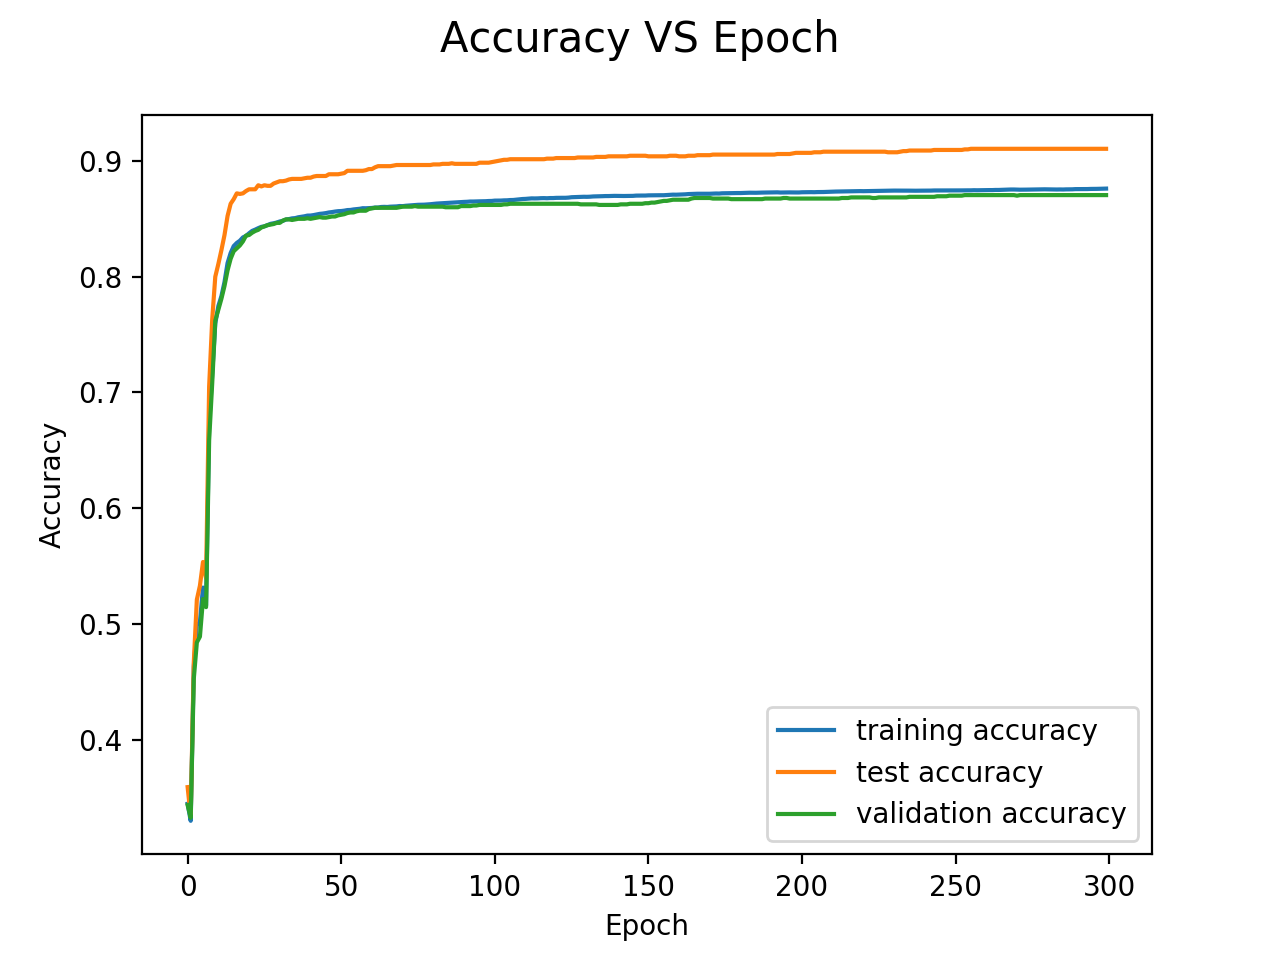
\includegraphics[width=1.8in,height=1.8in]{../softmax/figs/accuracy.png}  }}%
	\qquad
	\subfloat[label 2]{{	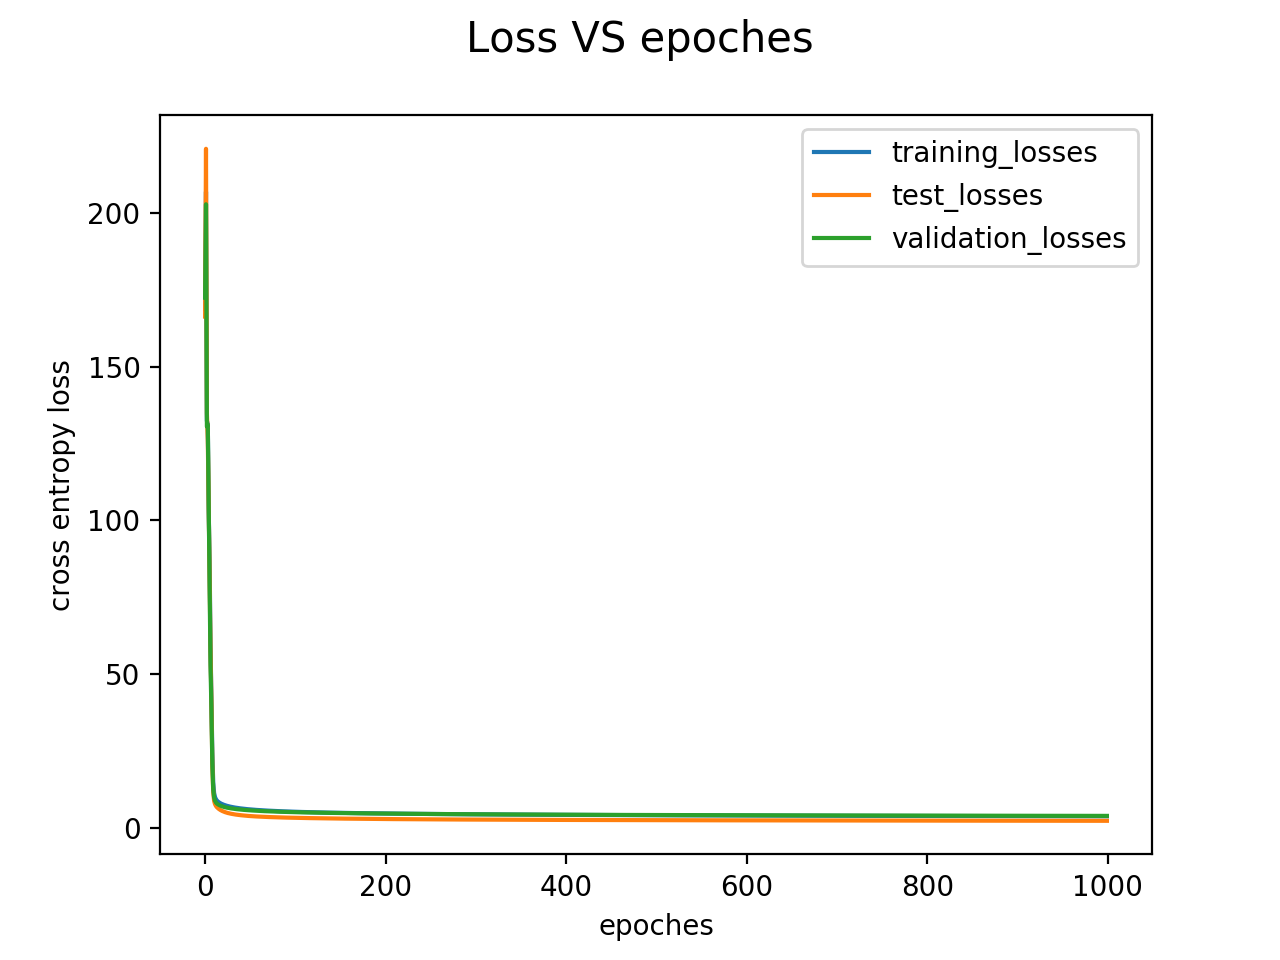
\includegraphics[width=1.8in,height=1.8in]{../softmax/figs/loss.png}  }}%
	\caption{2 Figures side by side}%
	\label{fig:example}%
\end{figure}



(b) In this experiement, we use  $L_2$ regularization with $\lambda = 0.01$. The figure is shown in Fig \ref{figure: 1}. 


(c) In this experiement, we use  $L_2$ regularization with $\lambda = 0.01$. The figure is shown in Fig \ref{figure: 2}.

(d) We plot the results in Fig \ref{figure: 3}. We can see that the image of the weight and the corresponding image of the average digit is almost the same. The reason is that we classify the images based on the inner product of the pixesls with the weights. And the inner product is maximized when the angle between the weight and the image is zero. So we see that the image of the weight and the corresponding image of the average digit is similar.

\begin{figure}[h]
	\centering	
	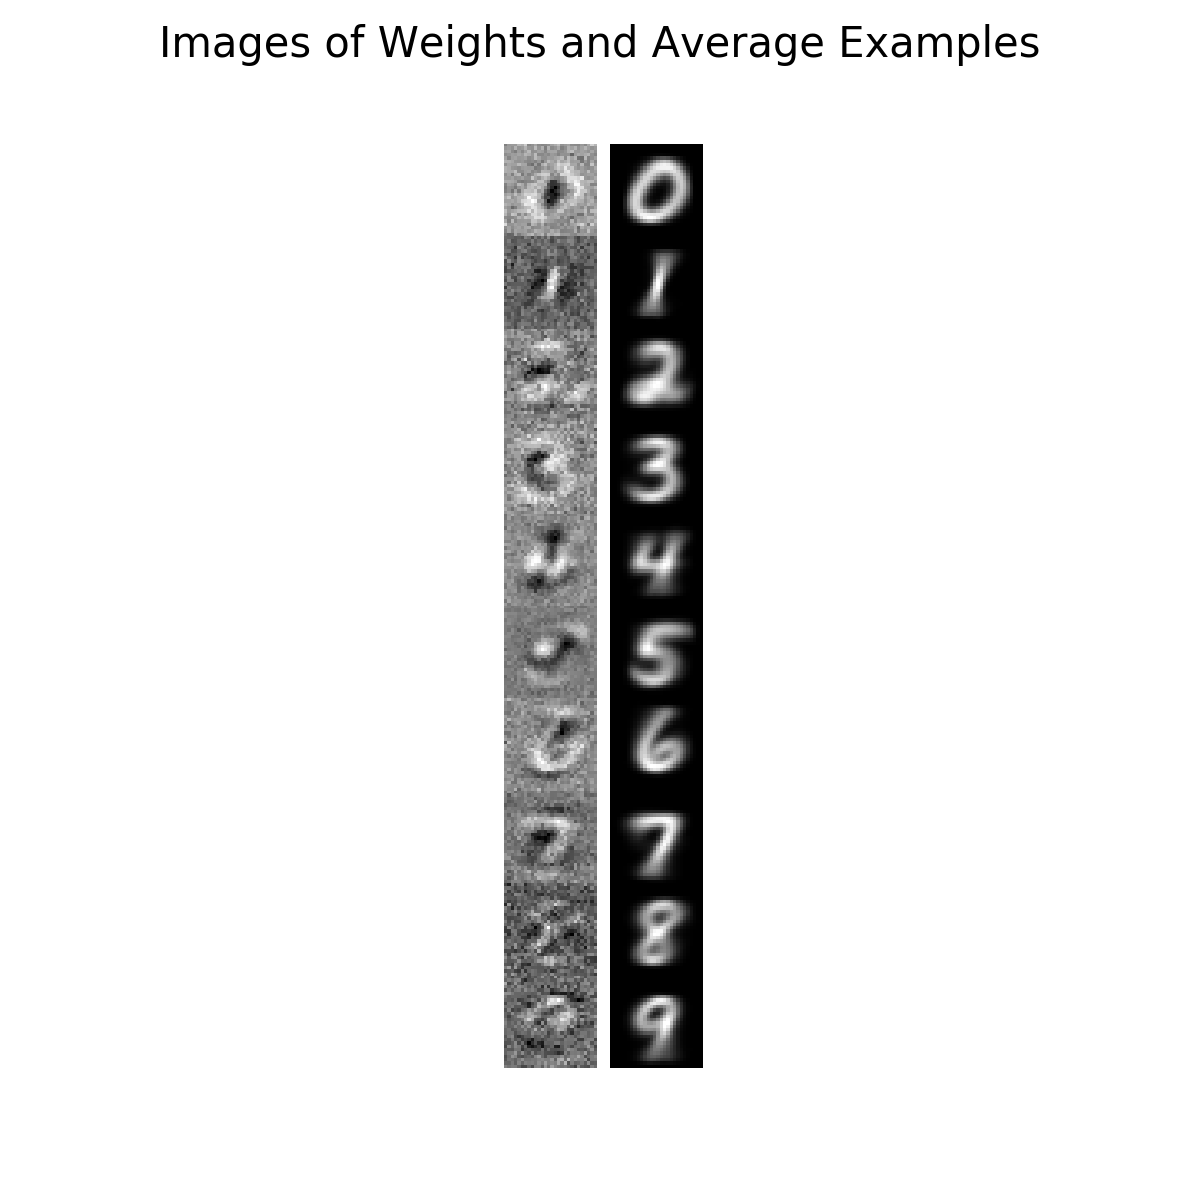
\includegraphics[width=2.8in,height=3.2in]{../softmax/figs/image_of_weights_and_digits.png} 
	\caption{}
	\label{figure: 3}
\end{figure}

\subsection{Discussion}




\subsubsection*{Acknowledgments}

. 

\subsubsection*{References}

\end{document}